\section[
  \texttt{NN}-level clock $+$ $2$-level system
]{%
  Page--Wootters model: \texttt{NN}-level clock $+$ $2$-level system\footnote{
    Here the symbol \texttt{NN} is used instead of \texttt{N} to avoid confusion with
    Mathematica's \emph{function} \texttt{N[]} which
    is used to convert symbolic expressions to their numerical value.
  }
}
\label{appendix:n-level}

\begin{Verbatim}
NN := 32
\end{Verbatim}

\begin{Verbatim}
T := DiagonalMatrix[Range[0,NN-1]] * \[Pi] / 16
\end{Verbatim}

\begin{Verbatim}
F := FourierMatrix[NN]
\end{Verbatim}

For simplicity, $\hbar = \omega = 1$

\begin{Verbatim}
\[CapitalOmega] := F.T.F\[ConjugateTranspose]  * 16 / \[Pi]
\end{Verbatim}

Hamiltonian in "ordinary" space
\begin{Verbatim}
Hs := \[ImaginaryI]{{0, 1}, {-1, 0}}
\end{Verbatim}
\begin{Verbatim}
MatrixForm[Hs]
\end{Verbatim}
\[
  \left(
    \begin{array}{cc}
     0 & i \\
     -i & 0 \\
    \end{array}
    \right)
\]

Matrix representation of \cite[eq. 1]{Lloyd:Time}.
We turn it into numeric (\verb!N[ ]!) as treating  it symbolically onwards would be unfeasible:
\begin{Verbatim}
J := N[KroneckerProduct[\[CapitalOmega],IdentityMatrix[2]] + KroneckerProduct[IdentityMatrix[NN],Hs]]
\end{Verbatim}
\begin{Verbatim}
Chop[Eigenvalues[J]]

Out[ ] = {32., 31., 30., 30., 29., 29., 28., 28., 27., 27., 26., 26., 25., 25., 24., 24., 23., 23., 22., 22., 21., 21., 20., 20., 19., 19., 18., 18., 17., 17., 16., 16., 15., 15., 14., 14., 13., 13., 12., 12., 11., 11., 10., 10., 9., 9., 8., 8., 7., 7., 6., 6., 5., 5., 4., 4., 3., 3., 2., 2., 1., 1., -1., 0}
\end{Verbatim}
\begin{Verbatim}
Eigenvalues[J][[40]]

Out[ ] = 12.

Eigenvalues[J][[41]]

Out[ ] = 11.

chosenEigenvector := Eigenvectors[J][[ 40]]

chosenEigenvectorB := Eigenvectors[J][[41]]

Normalization := Sqrt[Abs[chosenEigenvector[[1]]^2] + Abs[chosenEigenvector[[2]]^2] ]

NormalizationB := Sqrt[Abs[chosenEigenvectorB[[1]]^2] + Abs[chosenEigenvectorB[[2]]^2] ]

chosenEigenvectorNormalized  := chosenEigenvector / Normalization

chosenEigenvectorNormalizedB := chosenEigenvectorB / NormalizationB  

probability := Abs[chosenEigenvectorNormalized ^2]

probabilityB := Abs[chosenEigenvectorNormalizedB^2]

ListPlot[probability,
  GridLines ->{Range[0,NN*2, 2], Range[0, 1, 0.1]},
  AxesLabel->{n, "P(0), P(1)"},
  LabelStyle->Directive[16],
  PlotMarkers->{Automatic, 16},
  ImageSize->1024
]
\end{Verbatim}
\begin{figure}[!h]
  \centering
  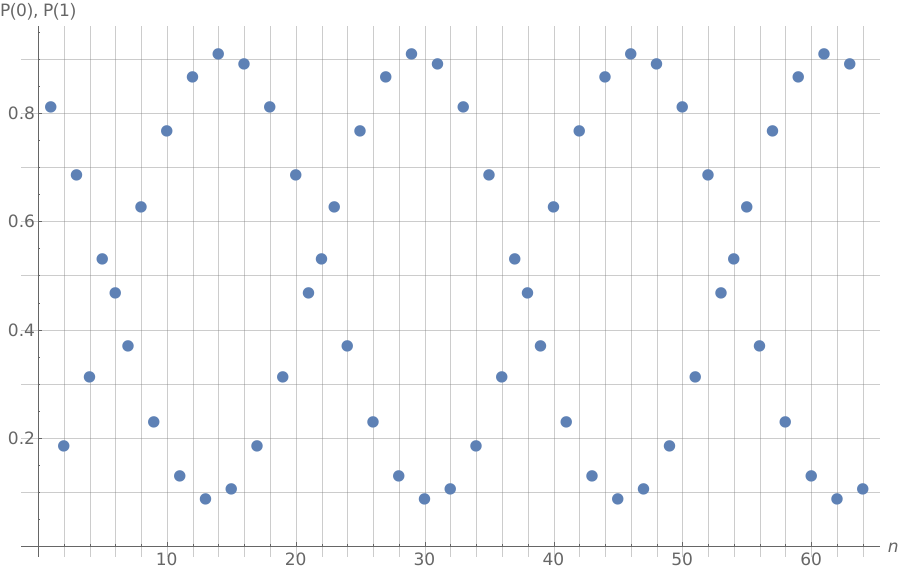
\includegraphics[width=.75\textwidth]{img/N32.png}
  \caption[]{png}{P-W ``evolution'' for $\hat{\mathbb{J}}$ eigenvalue $=12$}
\end{figure}  
\begin{Verbatim}

ListPlot[probabilityB,
  GridLines ->{Range[0,NN*2, 2], Range[0, 1, 0.1]},
  AxesLabel->{n, "P(0), P(1)"},
  LabelStyle->Directive[16],
  PlotMarkers->{Automatic, 16},
  ImageSize->1024
]
\end{Verbatim}
\begin{figure}[!h]
  \centering
  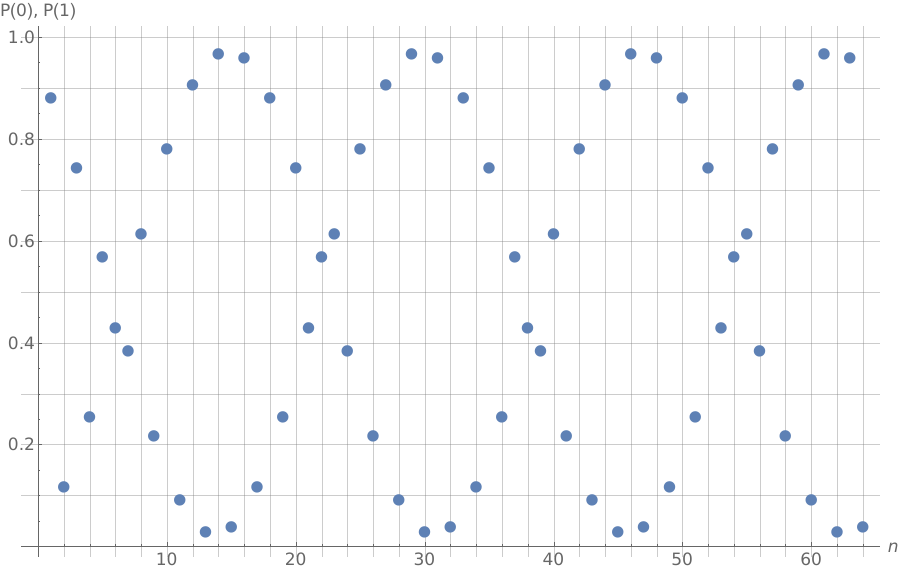
\includegraphics[width=.75\textwidth]{img/N32-B.png}
  \caption[]{png}{P-W ``evolution'' for $\hat{\mathbb{J}}$ eigenvalue $=11$}
\end{figure}

\subsection{Consistency of PW with ordinary QM (discrete approximation)}

\begin{Verbatim}
psi0 :=  chosenEigenvectorNormalizedB[[{1,2}]]
\end{Verbatim}

\begin{Verbatim}
psi[t_] := MatrixExp[-I Hs t, psi0 ]
\end{Verbatim}

\begin{Verbatim}
Plot[(Abs[psi[t]]^2)[[1]],{t,0,2\[Pi]},
  AxesLabel->{t, "P(0)"},
  LabelStyle->Directive[16],
  ImageSize->900
]
\end{Verbatim}
\begin{figure}[!h]
  \centering
  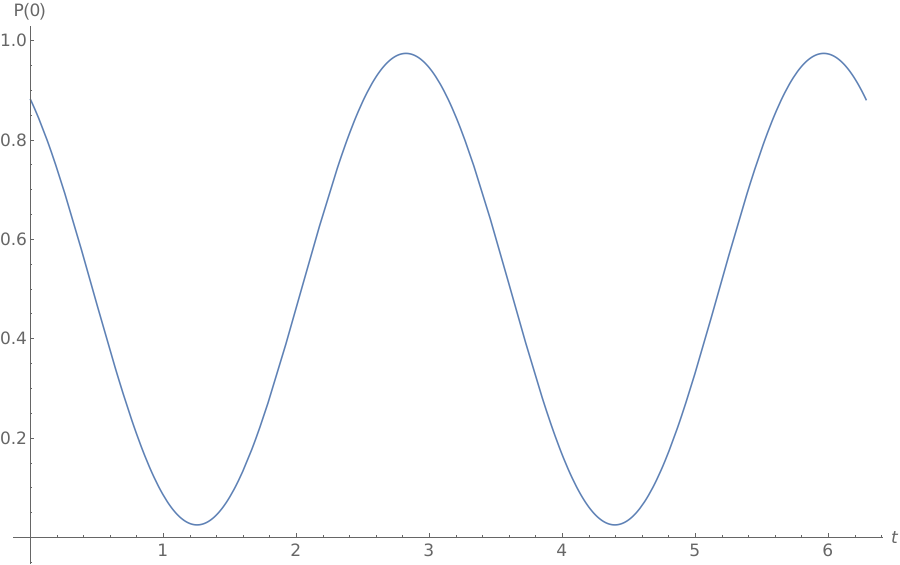
\includegraphics[width=0.75\textwidth]{img/probB_0.png}
  \caption[]{png}{
    Schr{\"o}dinger evolution of
    $\qty|\braket{0}{\psi(t)}|^2$, $t \in (0, 2\pi) $
    picking the first two components of an eigenvector of $\hat{\mathbb{J}}$
    as the two components of $\psi_{t=0}$ in ordinary Hilbert space.
    Related eigenvalue of $\hat{\mathbb{J}}$ is $11$
  }
\end{figure}

\begin{Verbatim}
Plot[(Abs[psi[t]]^2)[[2]],{t,0,2\[Pi]},
  AxesLabel->{t, "P(1)"},
  LabelStyle->Directive[16],
  ImageSize->900
]
\end{Verbatim}
\begin{figure}[!h]
  \centering
  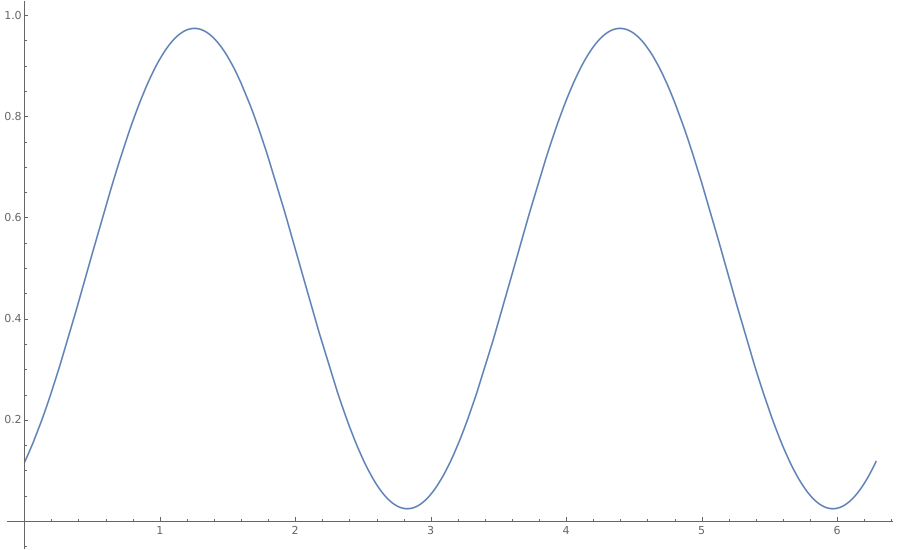
\includegraphics[width=0.75\textwidth]{img/probB_1.png}
  \caption[]{png}{
    Schr{\"o}dinger evolution of
    $\qty|\braket{1}{\psi(t)}|^2$, $t \in (0, 2\pi) $
    picking the first two components of an eigenvector of $\hat{\mathbb{J}}$
    as the two components of $\psi_{t=0}$ in ordinary Hilbert space.
    Related eigenvalue of $\hat{\mathbb{J}}$ is $11$
  }
\end{figure}

\subsubsection{Complex evolution of $\psi$ (not just $\qty|\psi|^2$)}

Please note index count is
$1, 2$ (cells above)
but refers, respectively, to computational base elements
$\ket{0}, \ket{1}$ in ordinary Hilbert space.
\begin{Verbatim}
re0psi[t_] := Simplify[Re[psi[t][[1]]], Assumptions->Element[t, Reals]]
im0psi[t_] := Simplify[Im[psi[t][[1]]], Assumptions->Element[t, Reals]]
re1psi[t_] := Simplify[Re[psi[t][[2]]], Assumptions->Element[t, Reals]]
im1psi[t_] := Simplify[Im[psi[t][[2]]], Assumptions->Element[t, Reals]]
\end{Verbatim}

\begin{Verbatim}
zAxis := ParametricPlot3D[{0,0,t}, {t,0,2\[Pi]}, PlotStyle->{Gray}]
psi0plot := ParametricPlot3D[{re0psi[t], im0psi[t], t}, {t, 0, 2\[Pi]}, PlotStyle->{Red} ]
psi1plot := ParametricPlot3D[{re1psi[t], im1psi[t], t}, {t, 0, 2\[Pi]}, PlotStyle->{Blue} ]
\end{Verbatim}

\begin{Verbatim}
Show[zAxis, psi0plot,psi1plot, ImageSize->Medium,
  AxesLabel -> {
    Style[Re["<0,1|\[Psi]>"], Bold],
    Style[Im["<0,1|\[Psi]>"], Bold],
    Style[t, Bold]
  }
]
\end{Verbatim}
\begin{figure}[!h]
  \centering
  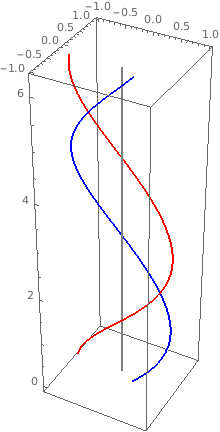
\includegraphics[width=0.25\textwidth]{img/qubit-evo-schrod.png}
  \caption[]{png}{
    Schr{\"o}dinger full complex evolution of components
    $\braket{0}{\psi(t)}$ (red) and 
    $\braket{1}{\psi(t)}$ (blue) for
    $t \in (0, 2\pi) $. The initial state
    has been chosen as the first two components of an eigenstate of
    $\hat{\mathbb{J}}$, related to eigenvalue $= 11$.
  }
\end{figure}

\begin{Verbatim}
pi = N[\[Pi]]

3.14159
\end{Verbatim}

\begin{Verbatim}
rephased[k_] := chosenEigenvectorNormalizedB [[k]] * Exp[-\[ImaginaryI]*pi*11*(k-1)/NN]

rephased1[k_] := chosenEigenvectorNormalizedB [[k]] * Exp[-\[ImaginaryI]*pi*11*(k-2)/NN]

scatter[k_] := {Re[ rephased[k]], Im[ rephased[k]], pi*(k-1)/NN}

scatter1[k_] := {Re[ rephased1[k]], Im[ rephased1[k]], pi*(k-2)/NN}

scatterPoints = Map[scatter, Range[1,2*NN, 2]]

Out[ ] = {{0.891003,-0.00706481,0.}, {0.896671,-0.0925068,0.19635}, {0.86788,-0.174394,0.392699}, {0.805737,-0.249579,0.589049}, {0.71263,-0.315173,0.785398}, {0.592137,-0.368655,0.981748}, {0.448889,-0.40797,1.1781}, {0.28839,-0.431607,1.37445}, {0.116809,-0.438657,1.5708}, {-0.0592618,-0.42885,1.76715}, {-0.233055,-0.402563,1.9635}, {-0.397892,-0.360805,2.15984}, {-0.547438,-0.305182,2.35619}, {-0.675946,-0.237831,2.55254}, {-0.778478,-0.16134,2.74889}, {-0.851094,-0.0786487,2.94524}, {-0.891003,0.00706481,3.14159}, {-0.896671,0.0925068,3.33794}, {-0.86788,0.174394,3.53429}, {-0.805737,0.249579,3.73064}, {-0.71263,0.315173,3.92699}, {-0.592137,0.368655,4.12334}, {-0.448889,0.40797,4.31969}, {-0.28839,0.431607,4.51604}, {-0.116809,0.438657,4.71239}, {0.0592618,0.42885,4.90874}, {0.233055,0.402563,5.10509}, {0.397892,0.360805,5.30144}, {0.547438,0.305182,5.49779}, {0.675946,0.237831,5.69414}, {0.778478,0.16134,5.89049}, {0.851094,0.0786487,6.08684}}

scatterPoints1 = Map[scatter1, Range[2,2*NN, 2]]

Out[ ] = {{0.116809,-0.438657,0.}, {-0.0592618,-0.42885,0.19635}, {-0.233055,-0.402563,0.392699}, {-0.397892,-0.360805,0.589049}, {-0.547438,-0.305182,0.785398}, {-0.675946,-0.237831,0.981748}, {-0.778478,-0.16134,1.1781}, {-0.851094,-0.0786487,1.37445}, {-0.891003,0.00706481,1.5708}, {-0.896671,0.0925068,1.76715}, {-0.86788,0.174394,1.9635}, {-0.805737,0.249579,2.15984}, {-0.71263,0.315173,2.35619}, {-0.592137,0.368655,2.55254}, {-0.448889,0.40797,2.74889}, {-0.28839,0.431607,2.94524}, {-0.116809,0.438657,3.14159}, {0.0592618,0.42885,3.33794}, {0.233055,0.402563,3.53429}, {0.397892,0.360805,3.73064}, {0.547438,0.305182,3.92699}, {0.675946,0.237831,4.12334}, {0.778478,0.16134,4.31969}, {0.851094,0.0786487,4.51604}, {0.891003,-0.00706481,4.71239}, {0.896671,-0.0925068,4.90874}, {0.86788,-0.174394,5.10509}, {0.805737,-0.249579,5.30144}, {0.71263,-0.315173,5.49779}, {0.592137,-0.368655,5.69414}, {0.448889,-0.40797,5.89049}, {0.28839,-0.431607,6.08684}}
\end{Verbatim}

\begin{Verbatim}
scatterPlot = ListPointPlot3D[scatterPoints, PlotStyle->{Red, PointSize[Large]}]
\end{Verbatim}
\begin{figure}[!h]
  \centering
  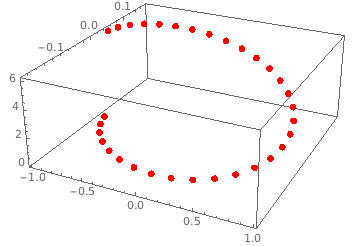
\includegraphics[width=0.4\textwidth]{img/scatterplot0.png}
  \caption[]{png}{
    Page--Wootters discrete-time evolution of
    $\braket{0}{\psi(t)}$ in 32 points between
    $t \in (0, 2\pi) $. From an eigenstate of
    $\hat{\mathbb{J}}$ related to eigenvalue $\epsilon = 11$.
    The evolution has been ``corrected'' via a phase oscillation
    factor $e^{-i \epsilon t}$
    as explained in \cite[\it ``The Zero-eigenvalue'']{Lloyd:Time}.
  }
\end{figure}

\begin{Verbatim}
scatterPlot1 = ListPointPlot3D[scatterPoints1, PlotStyle->{Blue, PointSize[Large]}]
\end{Verbatim}
\begin{figure}[!h]
  \centering
  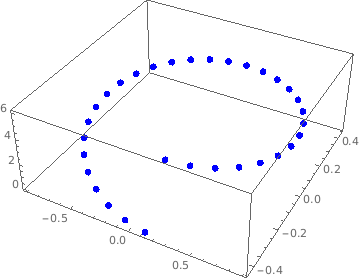
\includegraphics[width=0.4\textwidth]{img/scatterplot1.png}
  \caption[]{png}{
    Page--Wootters discrete-time evolution of
    $\braket{1}{\psi(t)}$ in 32 points between
    $t \in (0, 2\pi) $. From an eigenstate of
    $\hat{\mathbb{J}}$ related to eigenvalue $\epsilon = 11$.
    The evolution has been ``corrected'' via a phase oscillation
    factor $e^{-i \epsilon t}$
    as explained in \cite[\it ``The Zero-eigenvalue'']{Lloyd:Time}.
  }
\end{figure}

\begin{Verbatim}
Show[zAxis, psi0plot,psi1plot,scatterPlot, scatterPlot1, ImageSize->Large,
  AxesLabel->{
    Style[Re["<0,1|\[Psi]>"], Bold],
    Style[Im["<0,1|\[Psi]>"], Bold],
    Style[t, Bold]
  }
]
\end{Verbatim}
See Figure \ref{fig:complex-comparison}.